%%%%%%%%%%%%%%%%%%%%%%%%%%%%%%%%%%%%%%%%%%%%%%%%%%
\section{Analysis of ODE system}
%%%%%%%%%%%%%%%%%%%%%%%%%%%%%%%%%%%%%%%%%%%%%%%%%%
While numerical simulation of the full model reveals a range of blebbing behavior, we seek to elucidate how biophysical parameters determine the class of dynamics, specifically whether or not a bleb forms. To this end, we simplify the model by neglecting the tension term in Eq.~\ref{eq::nondimyM}. This transforms the force-balance equations Eq.~\ref{eq::nondimyM}-\ref{eq::nondimyC} into a pair of algebraic equations,
\begin{align}
y &= \frac{(a+cM)P}{a Mc + aP + McP}\label{eq::ODEyM}\\
y_C &= \frac{aP}{a MC + aP + McP}\label{eq::ODEyC},
\end{align}
 These are then substituted into the assembly/disassembly equations, yielding
\begin{align}
\frac{d c}{dt} &= \Omega a - c \label{eq::ODEC}\\
\epsilon \frac{d a}{dt} &= \frac{c}{1+c} \mbox{exp}\left( -\frac{1}{D} \frac{MPc}{a Mc + aP + McP}\right) \notag\\
 &- a\; \mbox{exp}\left( + \frac{1}{F}\frac{MPc}{a Mc + aP + McP}\right) \label{eq::ODEA}
\end{align}
\hspace{10pt}
The model is now a system of two ordinary differential equations (ODEs) amenable to phase plane analysis (Edelstein-Keshet, 1988). 

%%%%%%%%%%%%%%%%%%%%%%%%%%%%%%%%%%%%%%%%%%%%%%%%%%
\subsection{Regimes of behavior at small $\epsilon$}
%%%%%%%%%%%%%%%%%%%%%%%%%%%%%%%%%%%%%%%%%%%%%%%%%%

%%%%%%%%%%%%%%%%%%%%%%%%%%%%%%%%
\begin{figure}[htbp]
  \centering
  \label{fig:phasePlanes}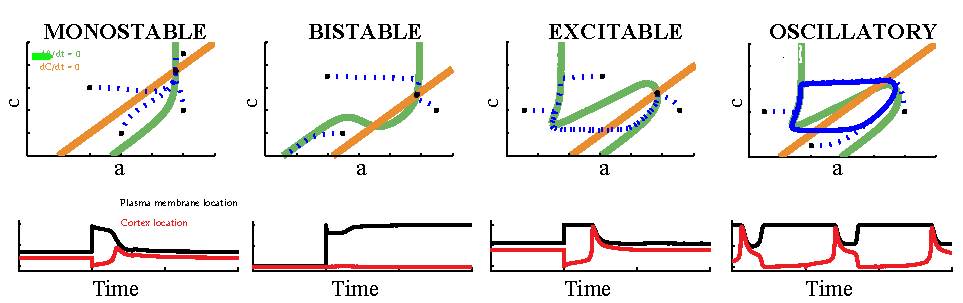
\includegraphics[width=13cm]{figs/figODERegimes.pdf}
  \caption{Phase plane analysis.}
\end{figure}
%%%%%%%%%%%%%%%%%%%%%%%%%%%%%%%%
Figure~\ref{fig:phasePlanes}



%%%%%%%%%%%%%%%%%%%%%%%%%%%%%%%%%%%%%%%%%%%%%%%%%%
\subsection{Bifurcation analysis in $\epsilon$ and $\Omega$}
%%%%%%%%%%%%%%%%%%%%%%%%%%%%%%%%%%%%%%%%%%%%%%%%%%

%%%%%%%%%%%%%%%%%%%%%%%%%%%%%%%%
\begin{figure}[htbp]
  \centering
  \label{fig:2DBifurcation}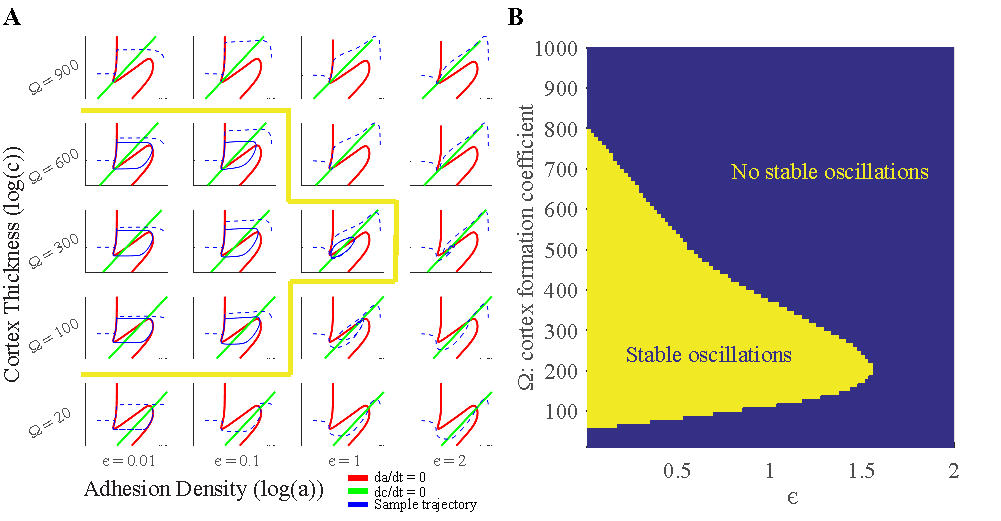
\includegraphics[width=13cm]{figs/2DBifurcation.pdf}
  \caption{A bifurcation in the ODE system. A) Phase plane diagrams with sample trajectories plotted for a range of $\Omega$ and $\epsilon$ values. The yellow line demarcates the boundary between the oscilatory and stable node regimes }
\end{figure}
%%%%%%%%%%%%%%%%%%%%%%%%%%%%%%%%
Figure~\ref{fig:2DBifurcation}

%%%%%%%%%%%%%%%%%%%%%%%%%%%%%%%%
\begin{figure}[htbp]
  \centering
  \label{fig:canard}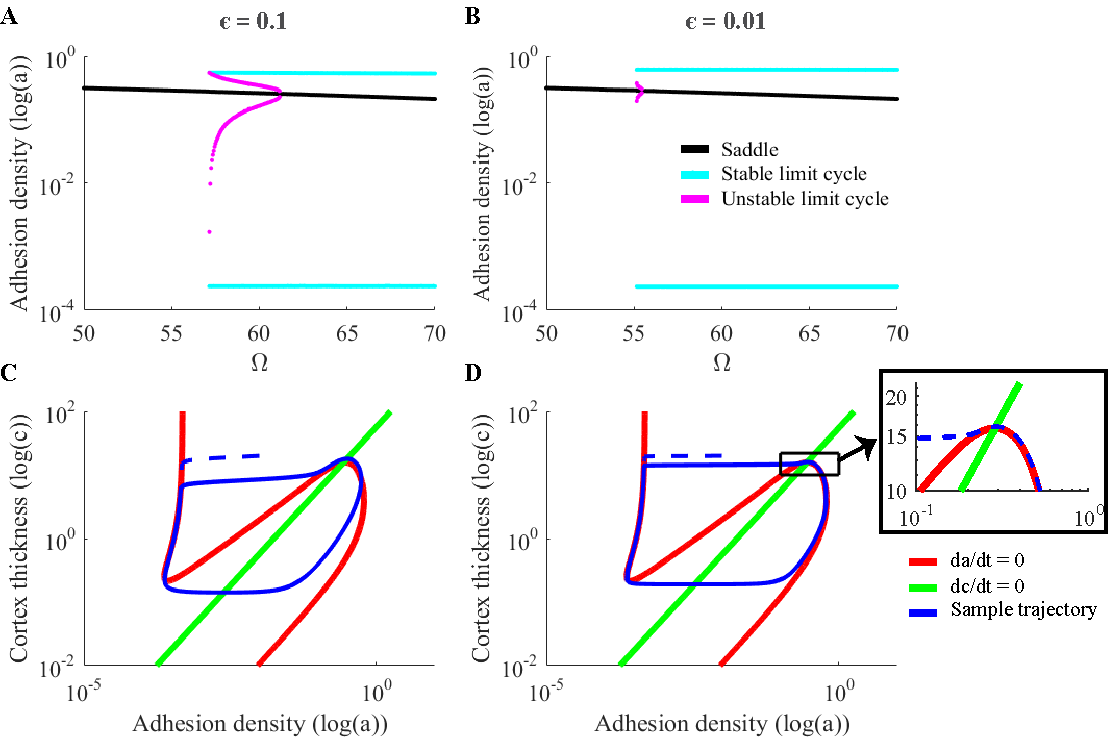
\includegraphics[width=13cm]{figs/figCanard.pdf}
  \caption{Canard explosion.}
\end{figure}
%%%%%%%%%%%%%%%%%%%%%%%%%%%%%%%%
The Duck in Figure~\ref{fig:canard}
